\documentclass[12pt]{beamer}
\definecolor{spoiler}{gray}{0.6}

\newcommand{\lib}[1]{\input{../../Libs/LaTeX/#1}}

\newcommand{\C}{\EuScript{C}}
\newcommand{\E}{\EuScript{E}}
\newcommand{\Le}{\mathcal{L}}

\newcommand{\btw}{\lessdot}
\newcommand{\mat}{\odot}
\newcommand{\ins}{\varpropto}
\newcommand{\g}{\mathfrak{g}}

\lib{Asymptote/Asymptote}
\lib{Graphics}
\lib{Math}


\usepackage{xcolor}
\usepackage{wrapfig}
\usepackage{lipsum}

\renewcommand{\O}{\mathcal{O}}
\renewcommand{\C}{\mathcal{C}}
\renewcommand{\S}{\mathcal{S}}
\renewcommand{\H}{\mathcal{H}}
\newcommand{\U}{\mathcal{U}}
\renewcommand{\N}{\mathcal{N}}

\newcommand{\vf}{\vspace{1mm}}

\newcommand{\cn}[1]{\mathrm{#1}}

\renewcommand{\r}[1]{{\color{red}{#1}}}
\renewcommand{\g}[1]{{\color{green}{#1}}}
\renewcommand{\b}[1]{{\color{blue}{#1}}}


\usepackage{color}

\DeclareMathOperator{\const}{const}

\usetheme{Ilmenau}

% \usecolortheme{whale}

\title[The Structure of Convexity]
	{\bfseries \LARGE The Structure of Convexity}
\author[Roman Maksimovich]{Roman Maksimovich}
\institute{Belgrade, Serbia}
\date{\today}

\def\fram#1#2{\begin{frame}\frametitle{\bf #1}#2\end{frame}}
\def\scolon{\rlap{,}\raisebox{0.8ex}{,} }
\def\mitem{\medskip\item}

\beamertemplatenavigationsymbolsempty

\begin{document}

\begin{frame}\titlepage\end{frame}

\newpage

\section*{Introduction}

\begin{frame}{Introduction}

    % \begin{wrapfigure}{r}{.5\textwidth}
    %     \centering

    \centering

    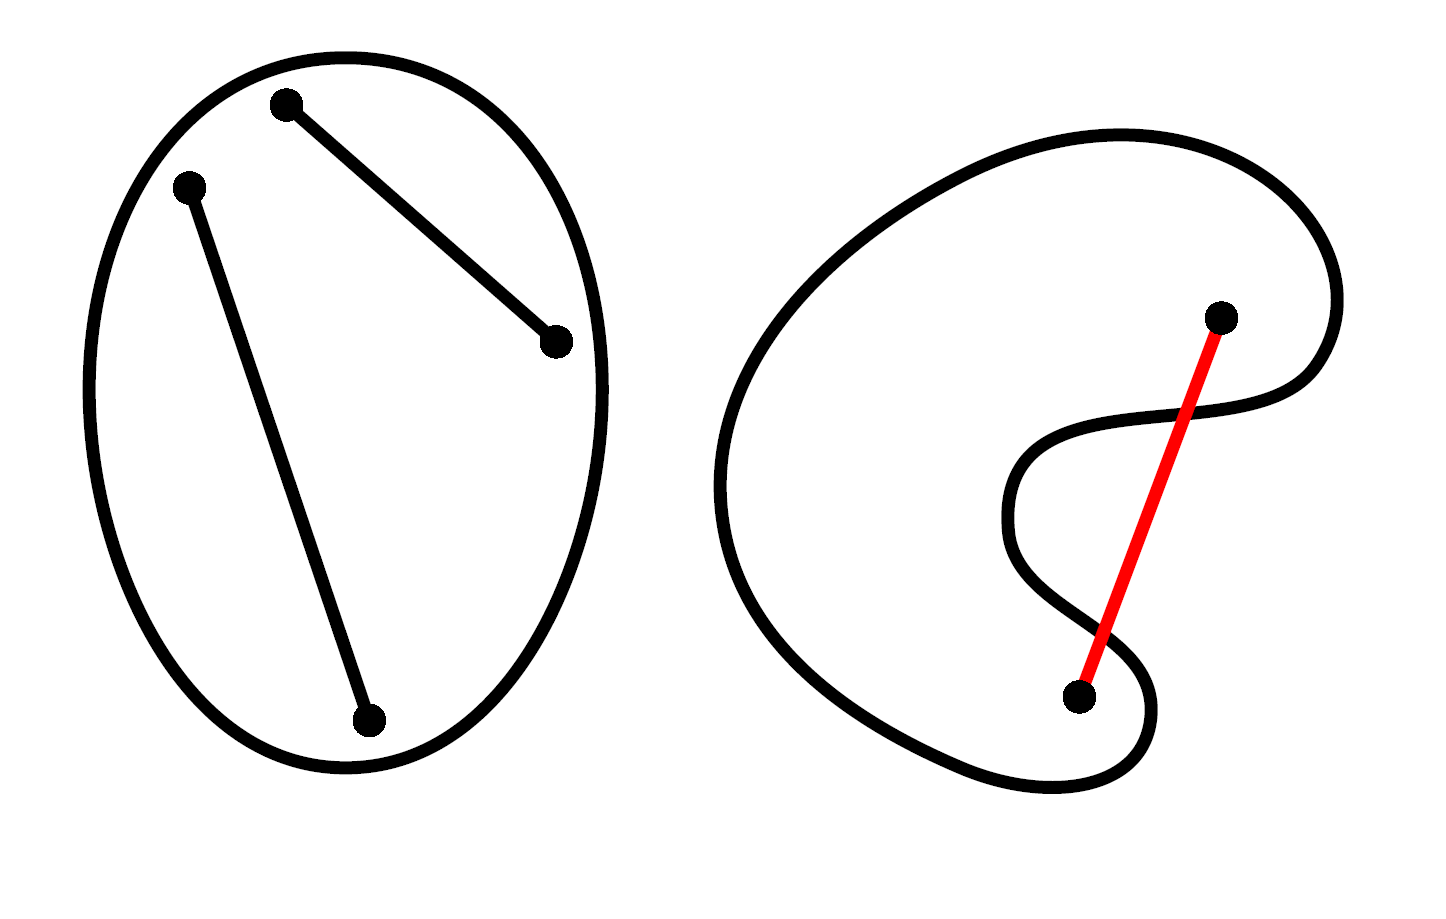
\includegraphics[width = 5cm]{1.png}

    % \end{wrapfigure}

    \begin{itemize}
        \item Convexity is an extremely popular concept.
        \item It is rarely studied as an abstract idea.
        \item 'Topology-like' proof methodology is pleasant.
    \end{itemize}

\end{frame}

\newpage

\section*{Internal theory}

\begin{frame}{Convex space}
    \begin{definition}
        \((X, \C)\) is a \textit{convex space} if:

        \begin{itemize}
            \item \(\varnothing\), \(X\) lie in \(\C\);
            \item For every \(\A \subset \C\) we have \(\bigcap \A \in \C\);
            \item For every \textit{net} \(\N \subset \C\) we have \(\bigcup \N \in \C\).  
        \end{itemize}
    \end{definition}

    \begin{definition}
        \textit{Convex hull} \(\tp{A}\) --- the smallest convex set containing \(A\).
    \end{definition}
\end{frame}

\newpage

\begin{frame}{Polytopes, freedom, dimension}
    \centering

    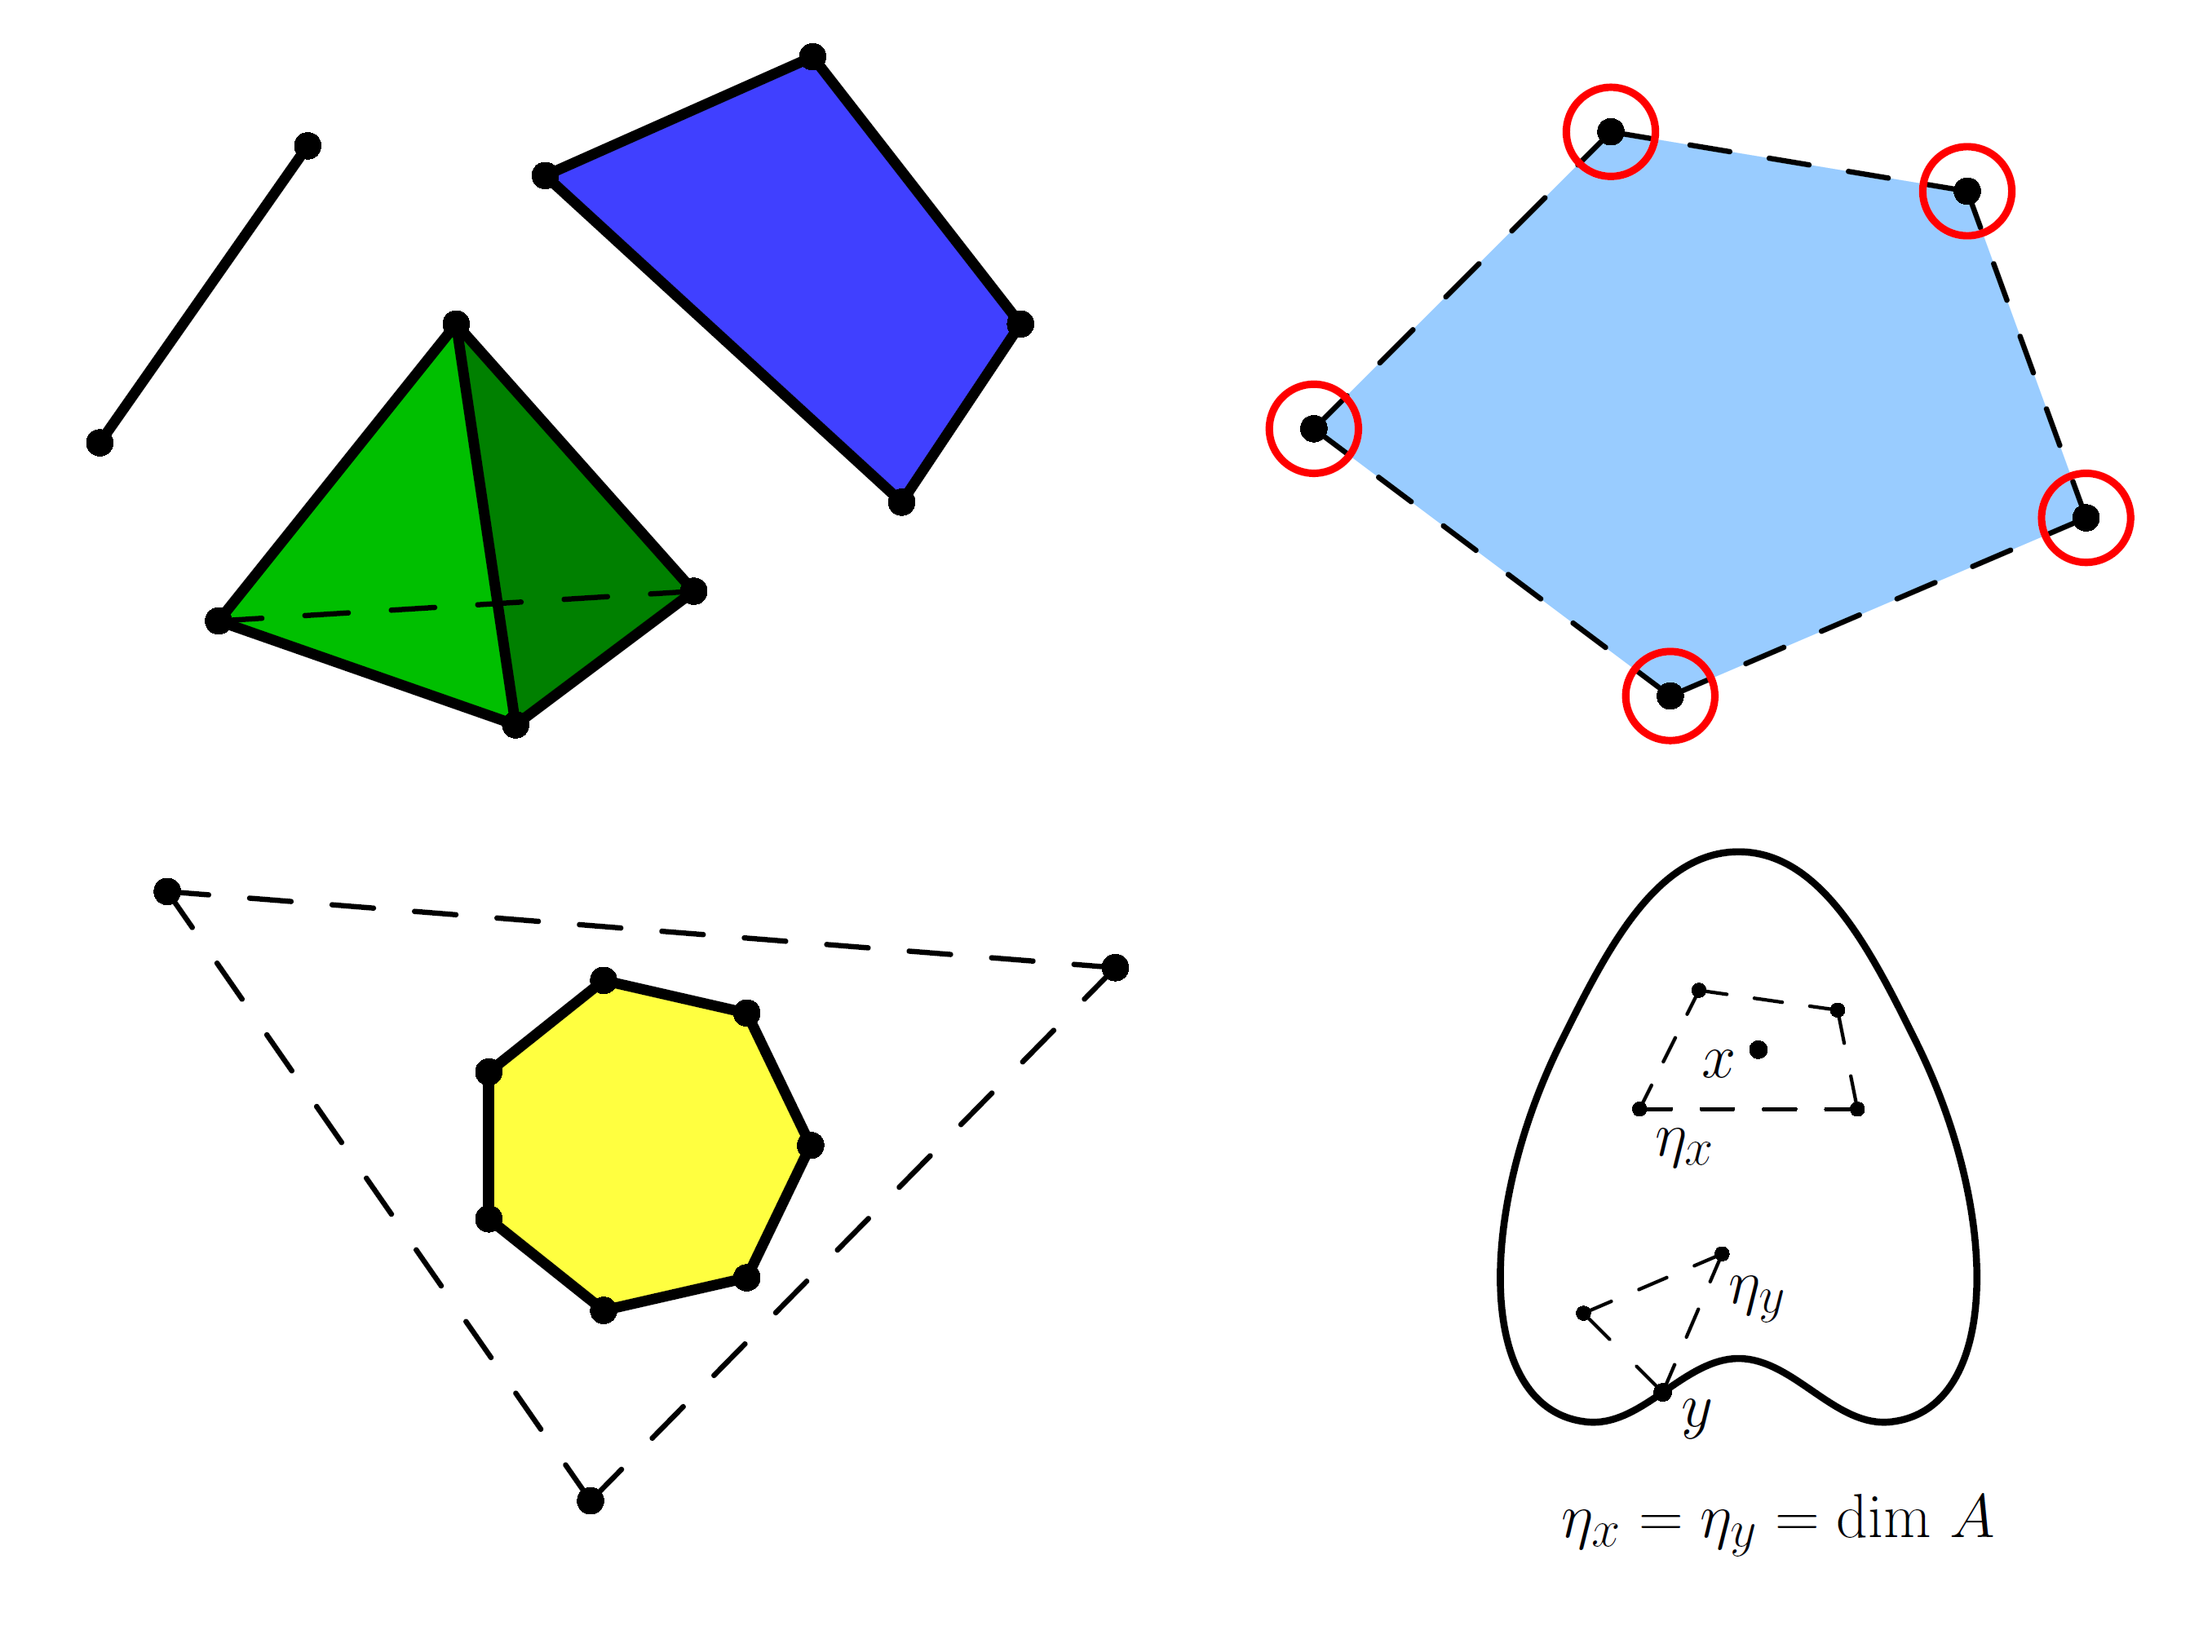
\includegraphics[width=9cm]{5.png}
\end{frame}

\newpage

\begin{frame}{Hyperplanes}
    \begin{definition}
        \textit{Hyperplane} --- union of a \textbf{maximal} net of polytopes of the same dimension.
    \end{definition}
    
    \centering

    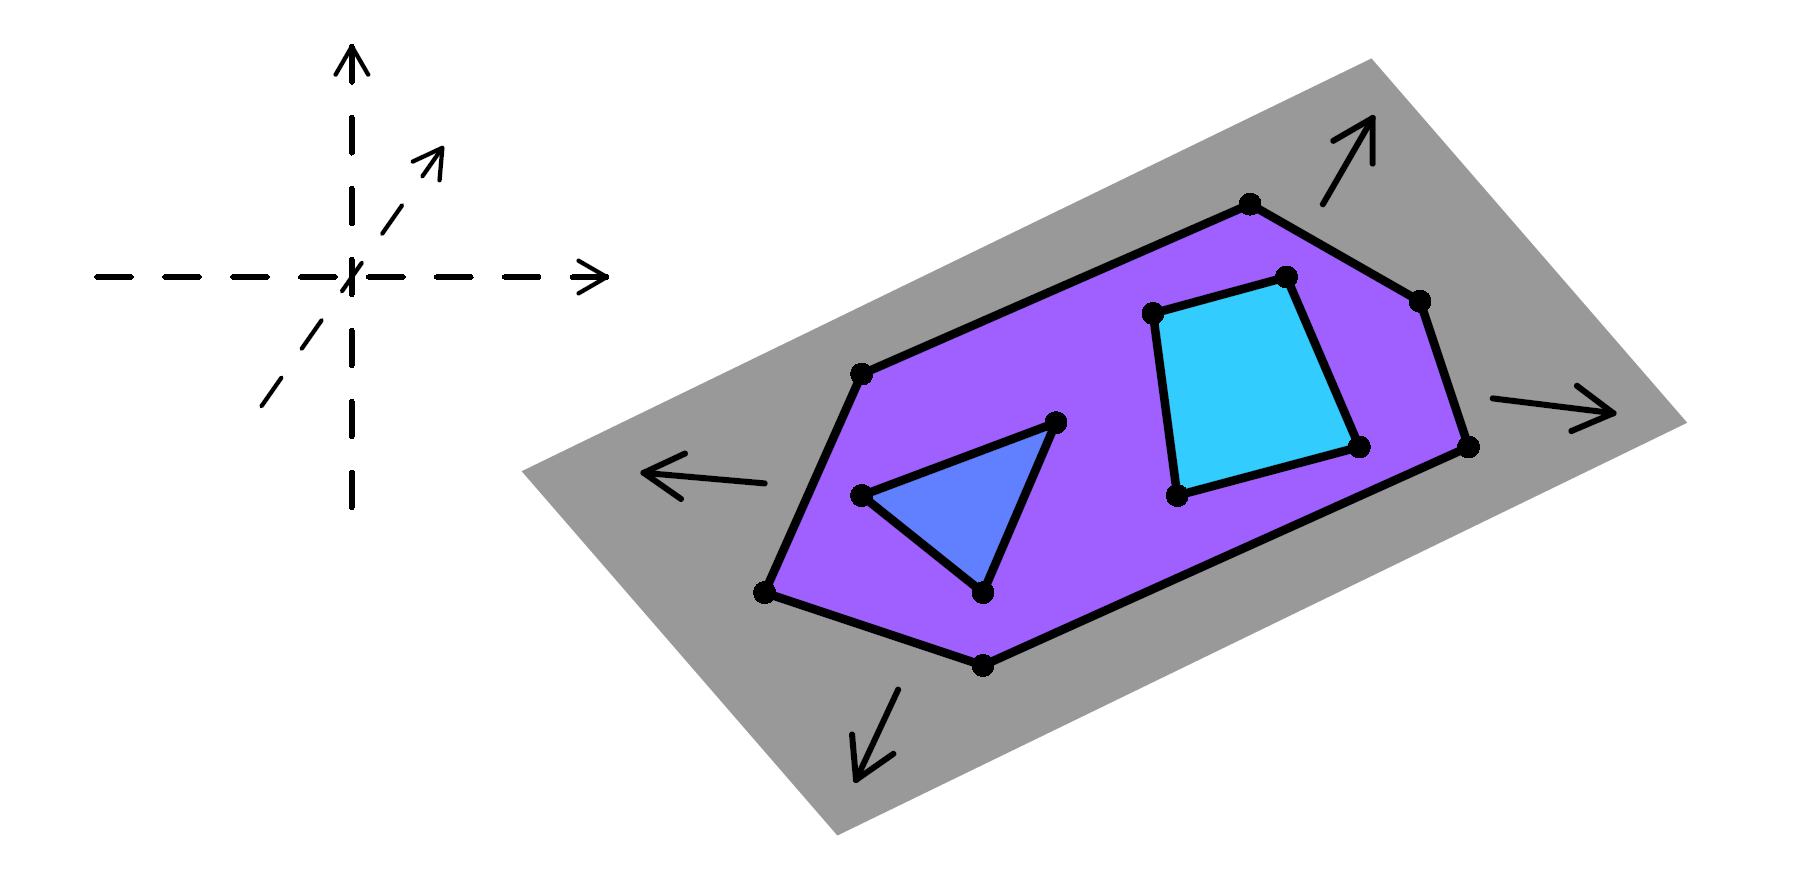
\includegraphics[width = 9.5cm]{7.png}
\end{frame}

\newpage

\begin{frame}{The Polytope Union Lemma}
    \begin{lemma}
        Let \(P\), \(Q\), \(L\) be polytopes of equal dimension, \(L \subset P \cap Q\). Then the dimension of \(\tp{P \cup Q}\) is \(m\).
    \end{lemma}

    \centering

    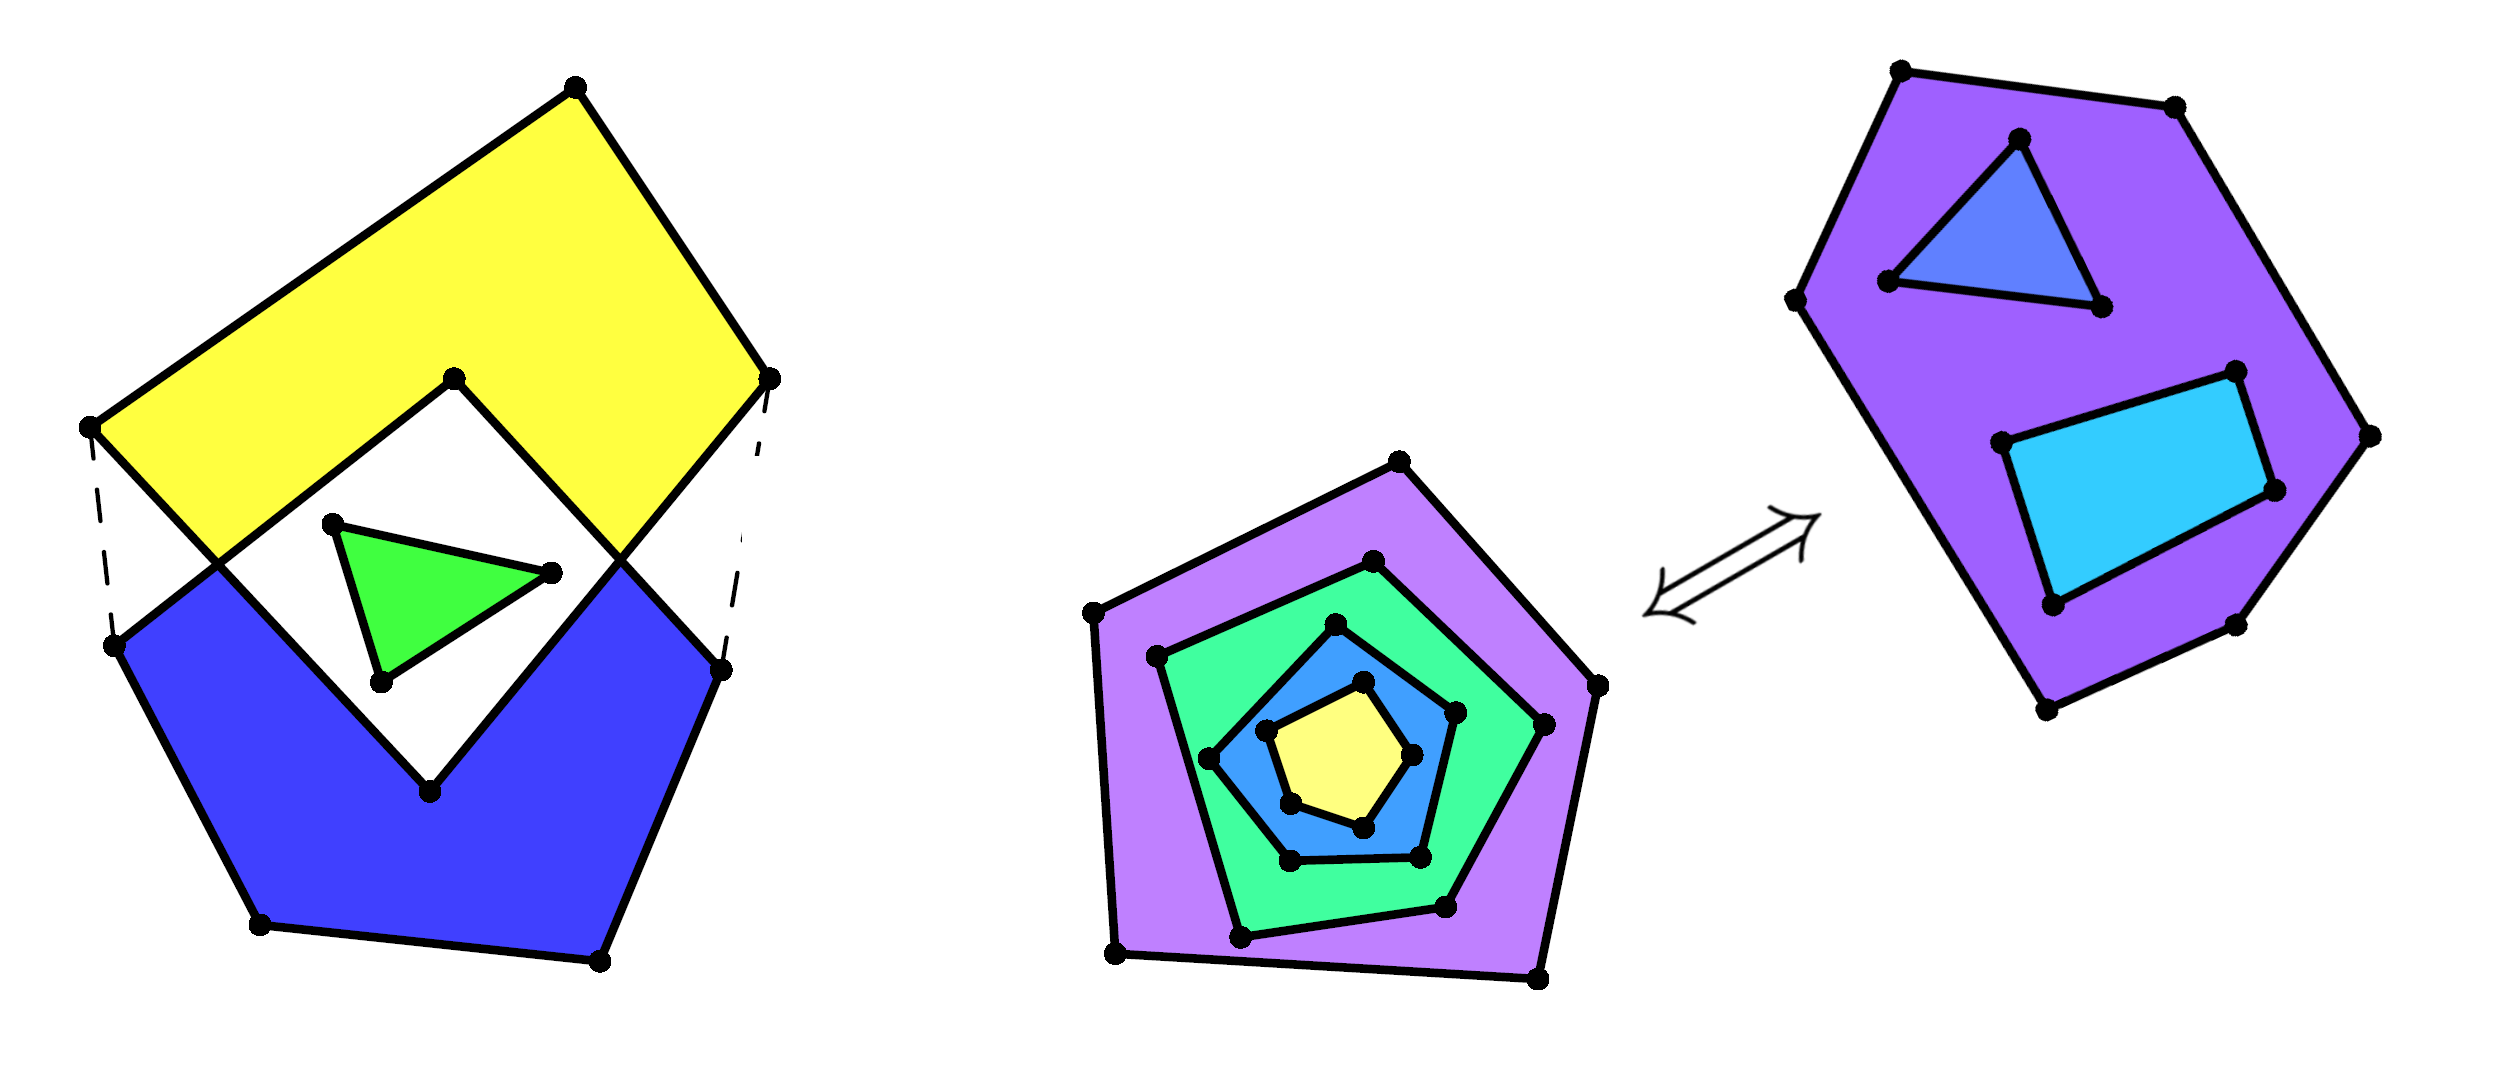
\includegraphics[width = 10.5cm]{8.png}
\end{frame}

\newpage



\section*{Inducing structures}

\begin{frame}{Order convexity}
    \centering

    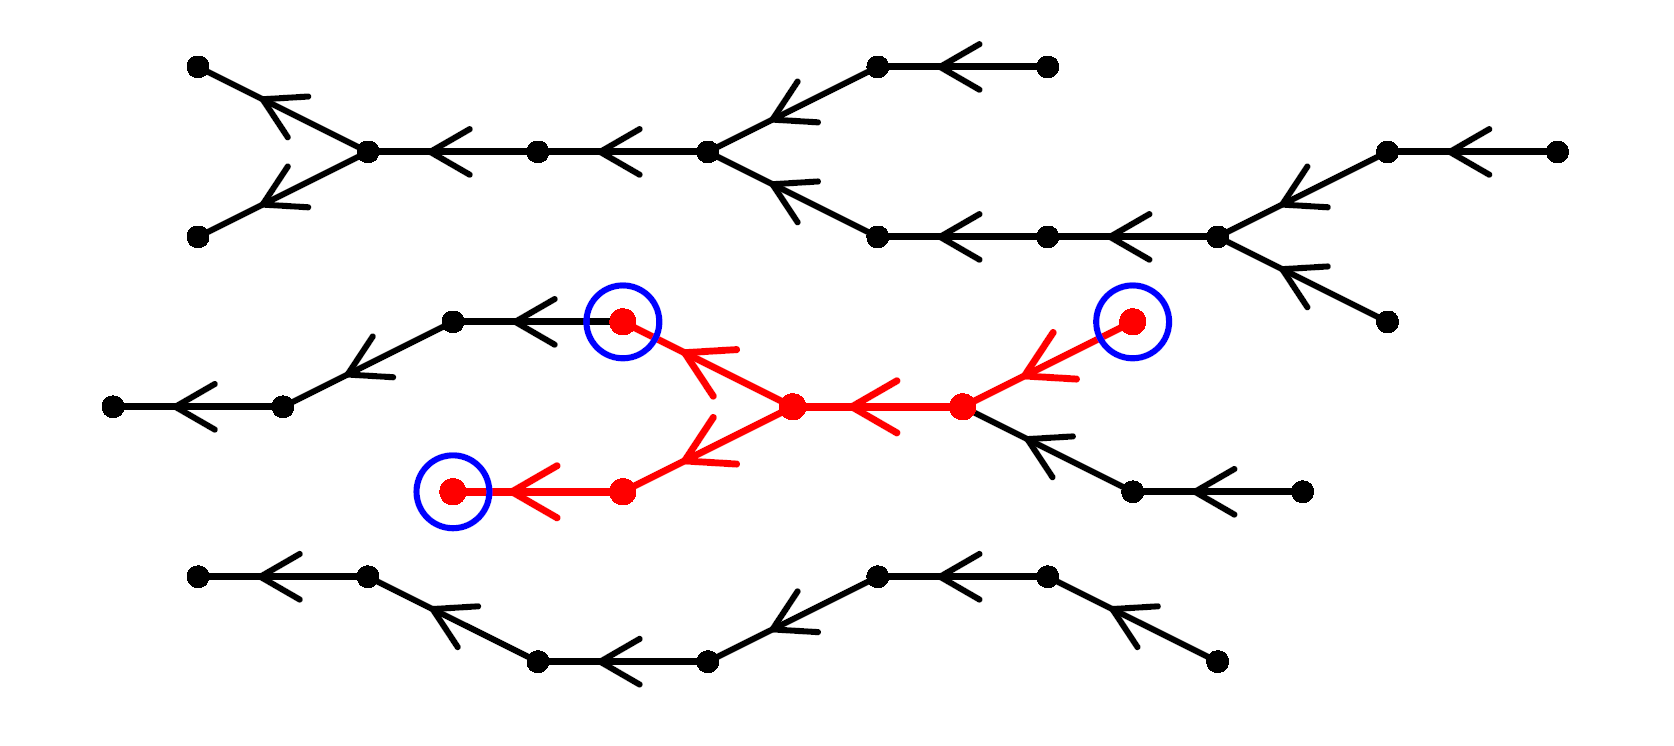
\includegraphics[width = 9cm]{9.png}

    \begin{theorem}
        Every ordered convex space is free, i.e. contains only free polytopes.
    \end{theorem}
\end{frame}

\newpage

\begin{frame}{\(n\)-Affinity}
    \begin{definition}
        1-Affine convex space \(\ \Longleftrightarrow \ \) each segment's convexity is induced by a linear order.
    \end{definition}

    \centering

    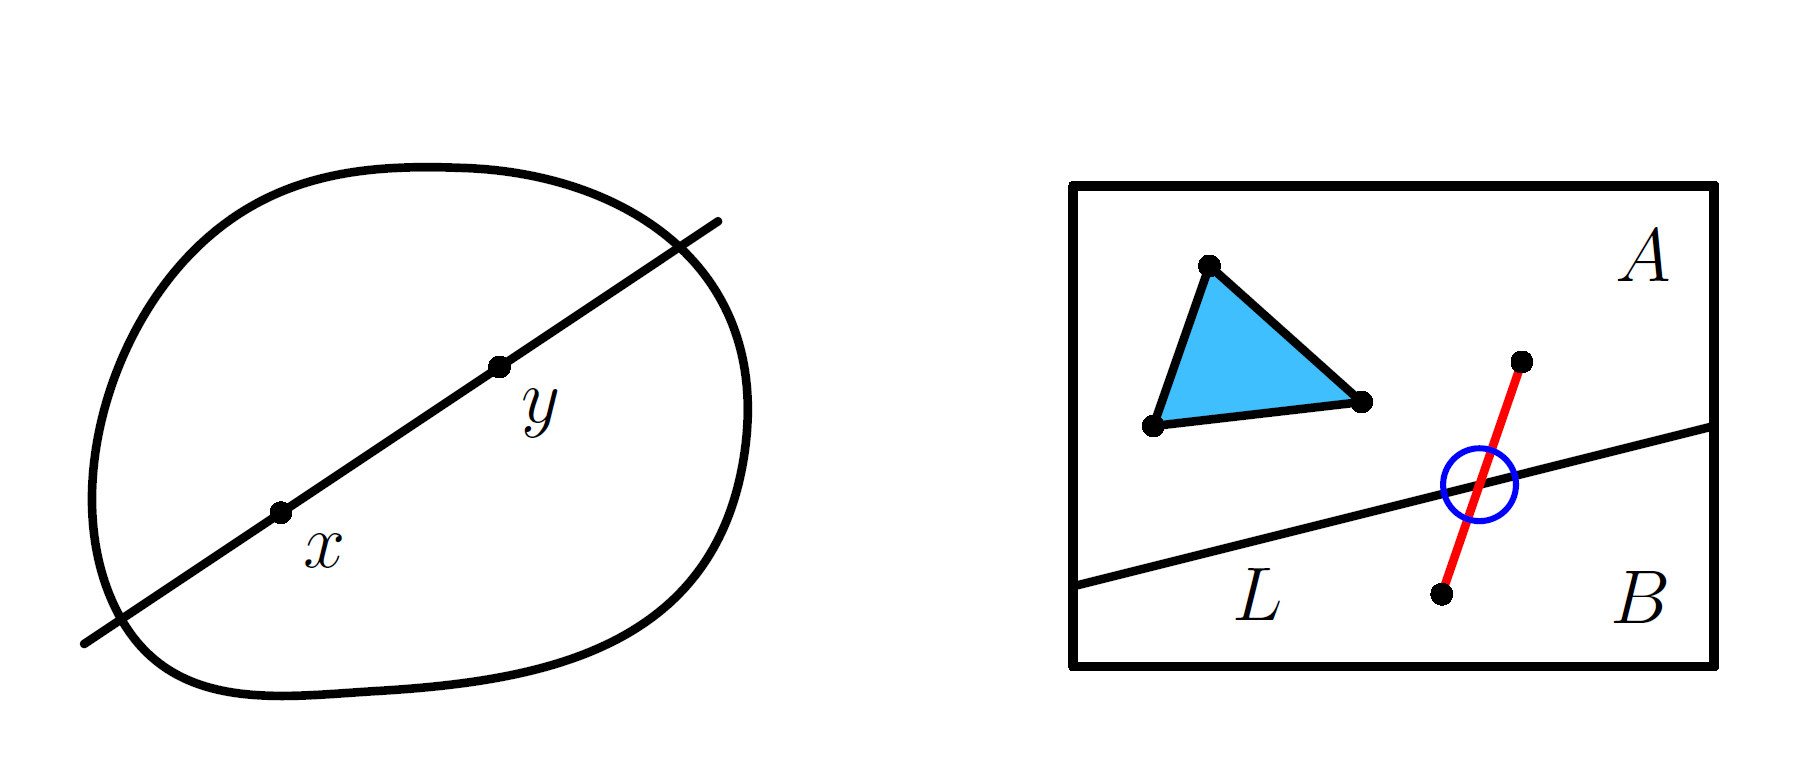
\includegraphics[width = 10.5cm]{10.png}
\end{frame}

\newpage

\begin{frame}{Metric convexity}
    \centering

    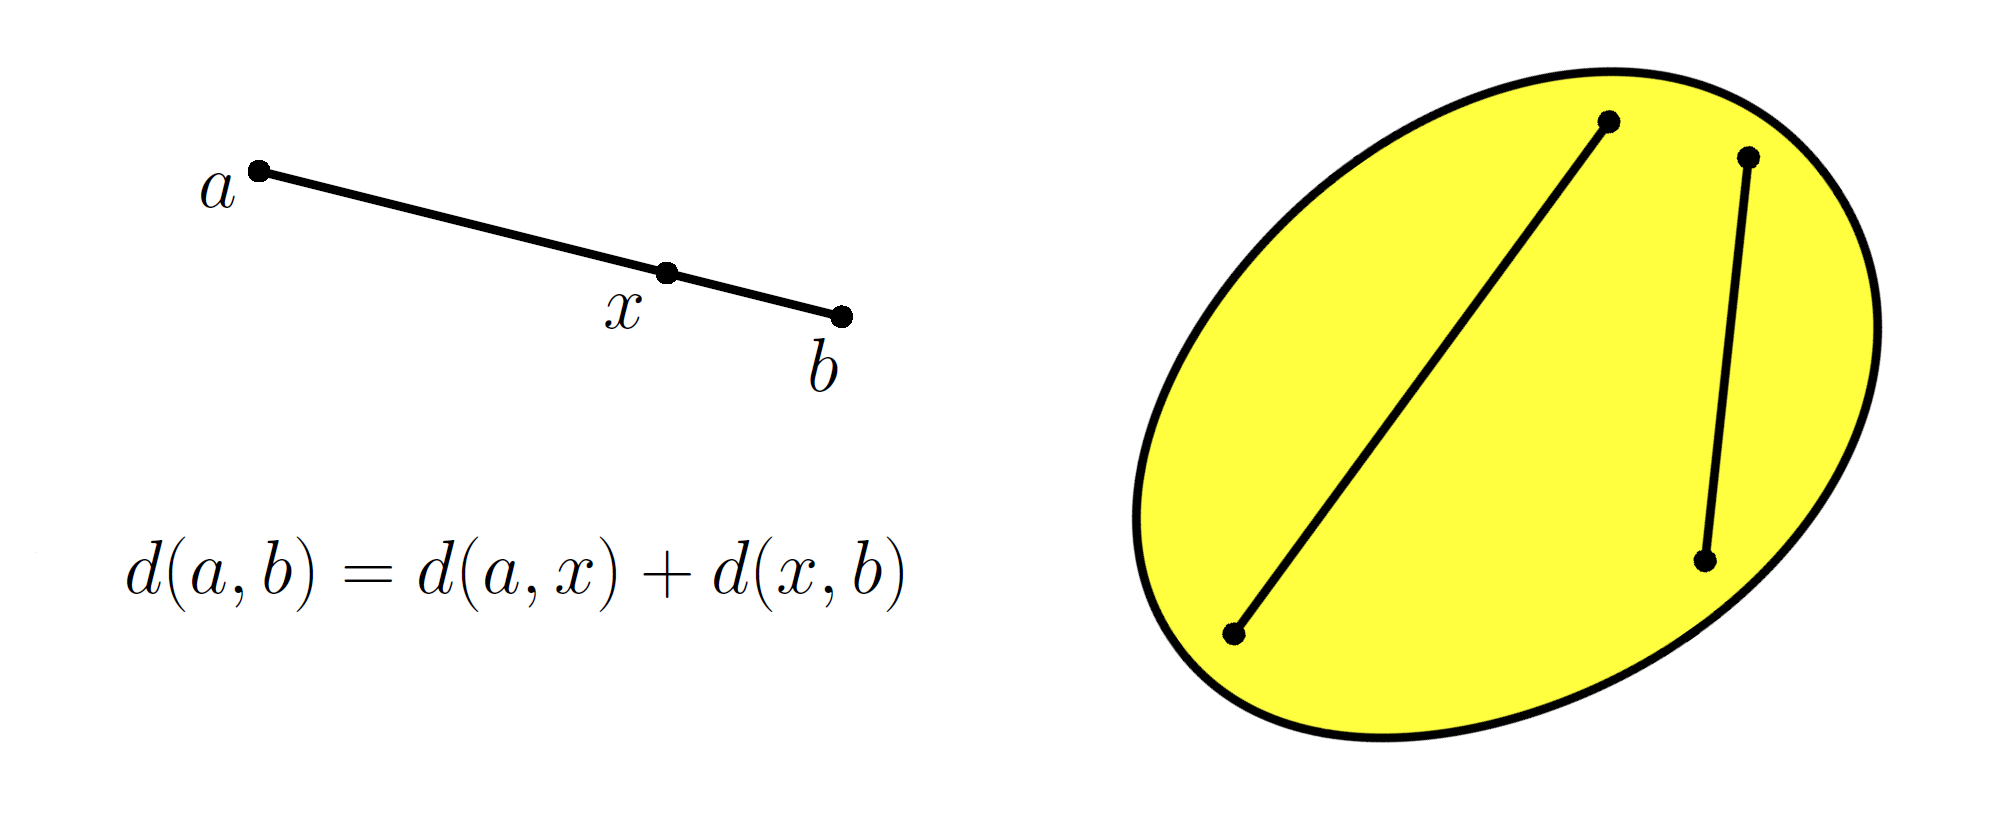
\includegraphics[width = 10cm]{11.png}

    \begin{definition}
        Convex \(\ \Longleftrightarrow \ \) contains the segment connecting every pair of points.
    \end{definition}
\end{frame}

\newpage

\begin{frame}{Join, Finite-segmentiality}
    \centering

    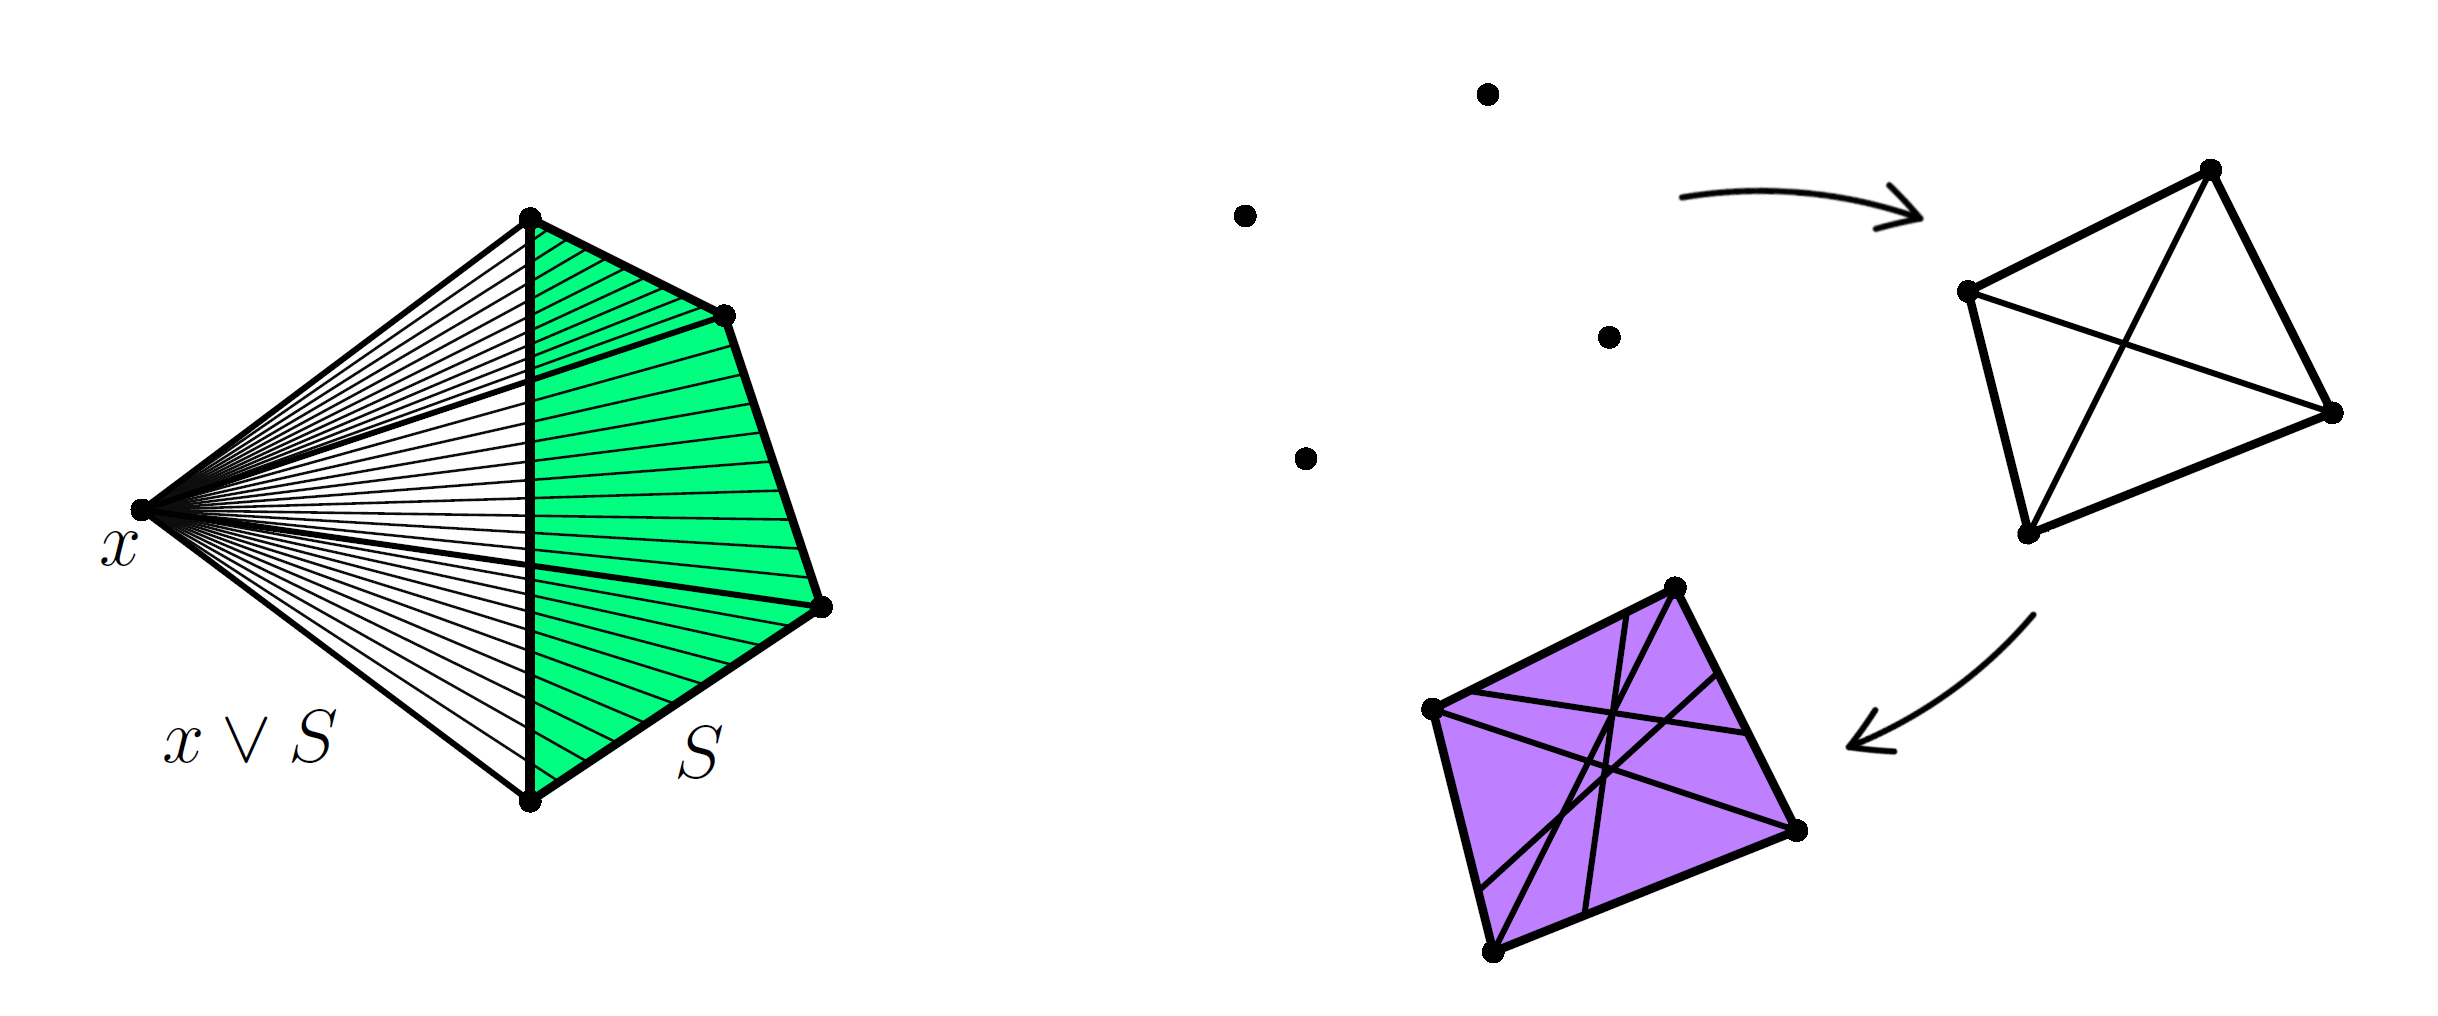
\includegraphics[width = 11cm]{12.png}

    \begin{theorem}
        2-Affine + TPUL + Finite-segmential \(\ \Longrightarrow \ \) Free.
    \end{theorem}
\end{frame}

\newpage


\section*{UGS}

\begin{frame}{Uniquely Geodesic Metric Spaces}
    \begin{definition}
        UGS: There is a unique path \(f\) such that \(|f| = d(a, b)\).
    \end{definition}

    \centering

    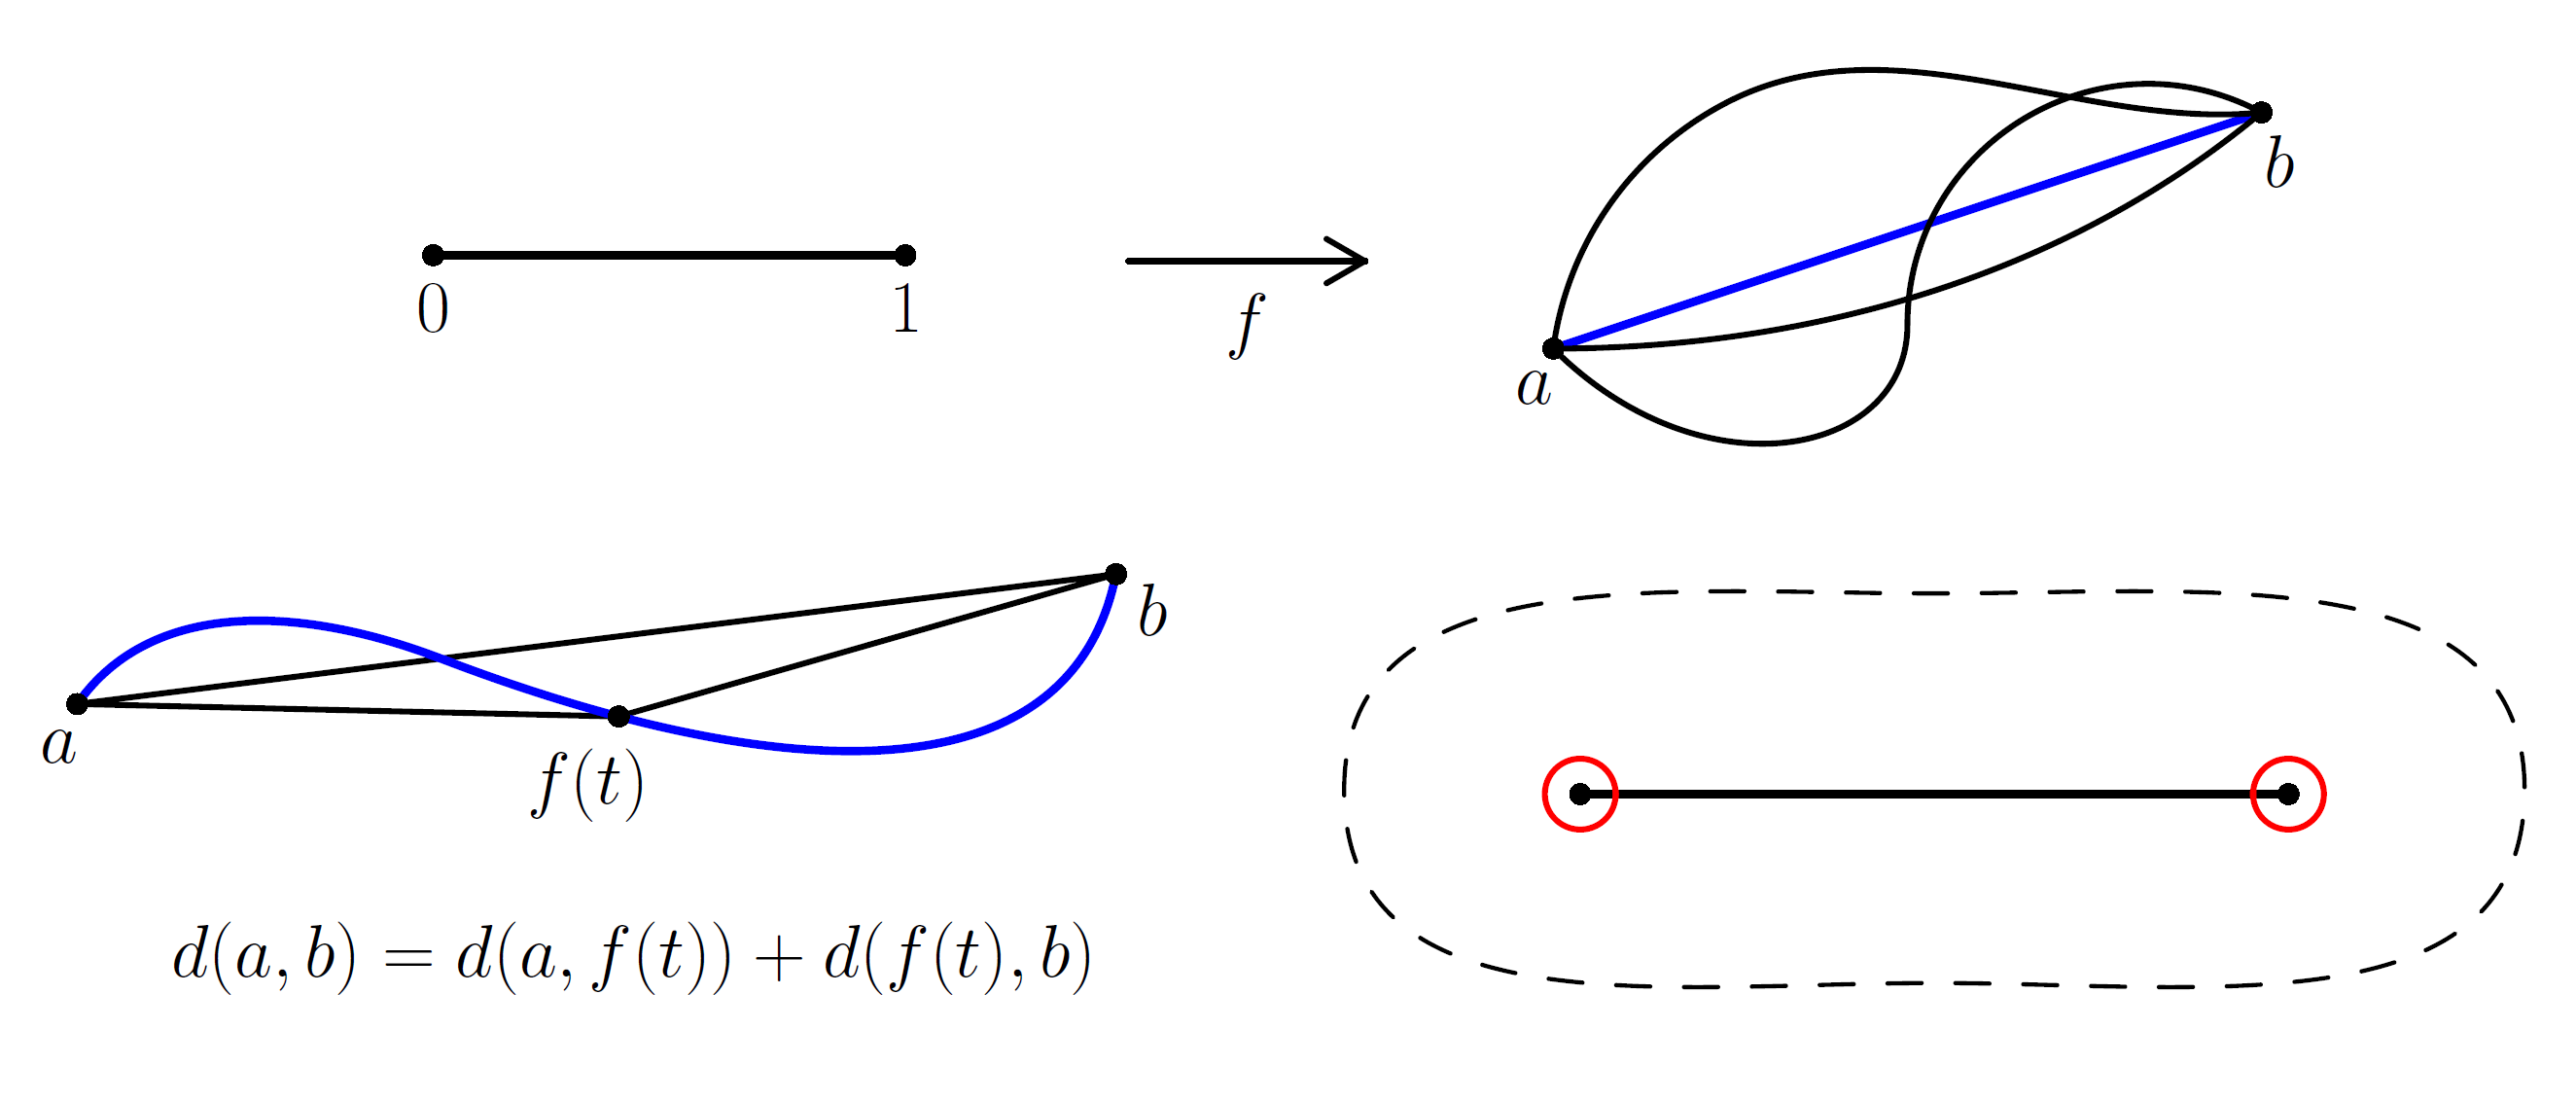
\includegraphics[width = 10.5cm]{13.png}
\end{frame}

\newpage

\section*{Induced structures}

\begin{frame}{The Polytope Intersection Lemma}
    \centering

    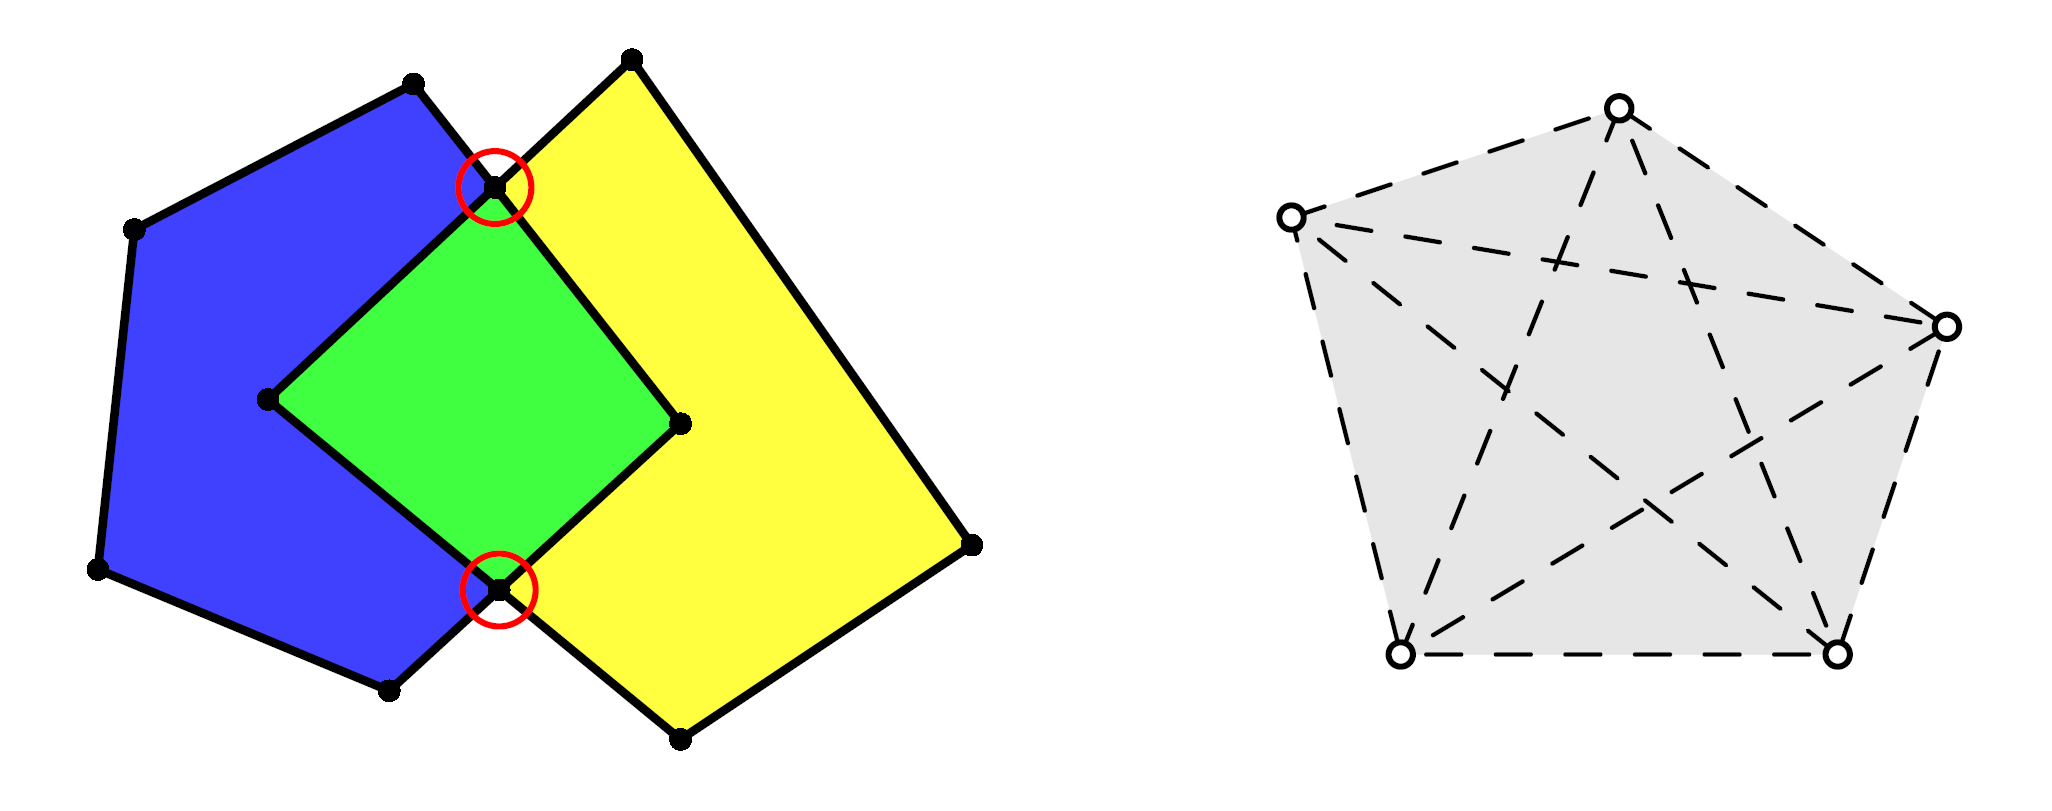
\includegraphics[width = 10cm]{14.png}

    \begin{definition}
        Free + Finite-dimensional + TPUL + TPIL \(\ \Longrightarrow \ \) Topology
    \end{definition}
\end{frame}

\newpage

\begin{frame}{Local convexity}
    % \begin{definition}
    %     The whole space may not be convex, but each point has a convex neighborhood.
    % \end{definition}
    
    \centering

    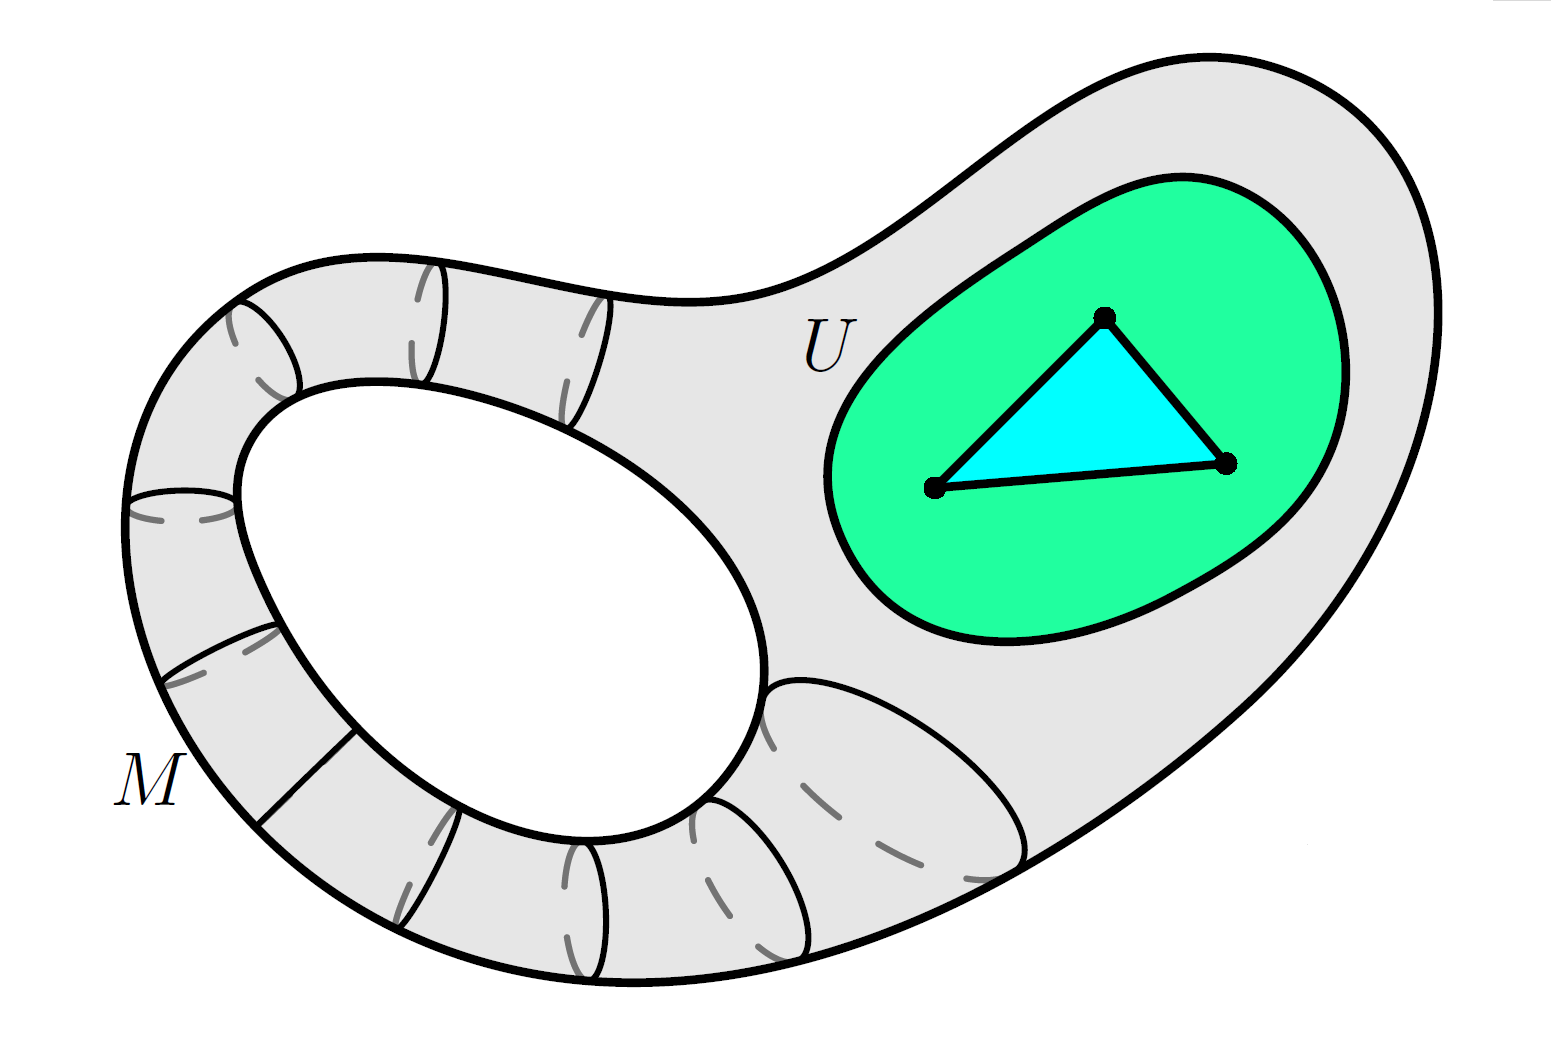
\includegraphics[width = 10cm]{15.png}
\end{frame}

\newpage

\begin{frame}{Local isomorphism}
    \begin{lemma}
        \(\R^2\) is not isomorphic to \(B^2\), but they are locally isomorphic.
    \end{lemma}

    \centering

    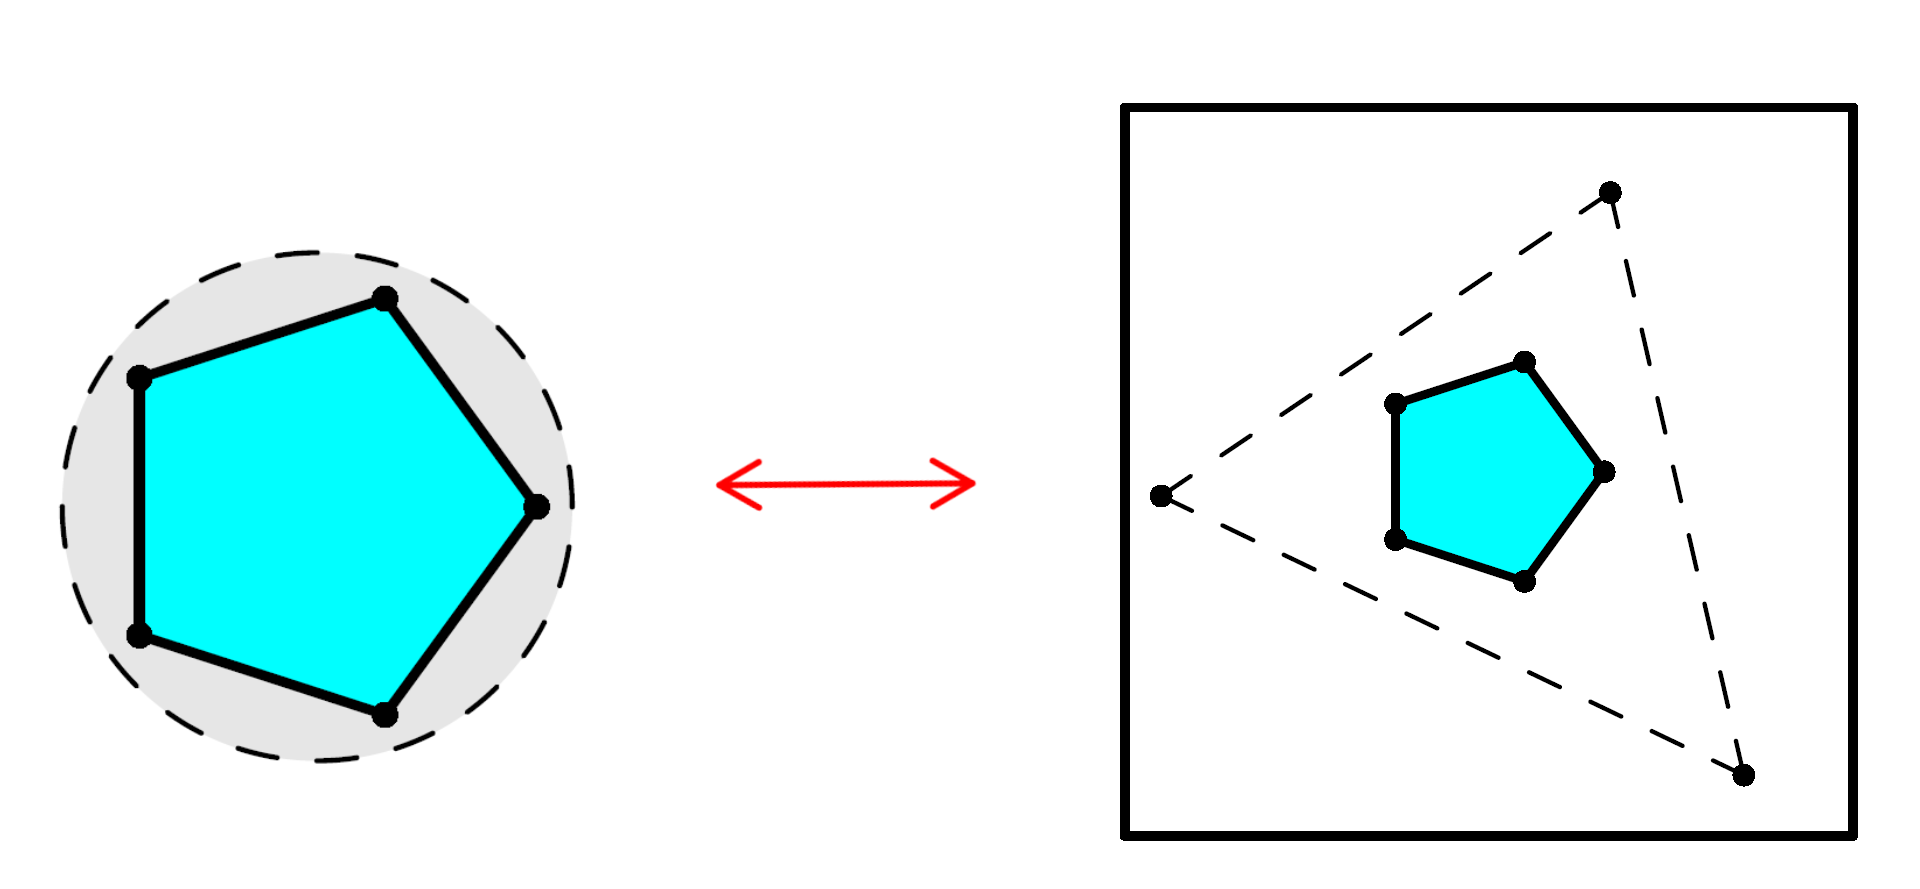
\includegraphics[width = 10cm]{17.png}
\end{frame}

\newpage

\begin{frame}{Riemannian manifolds}
    \centering

    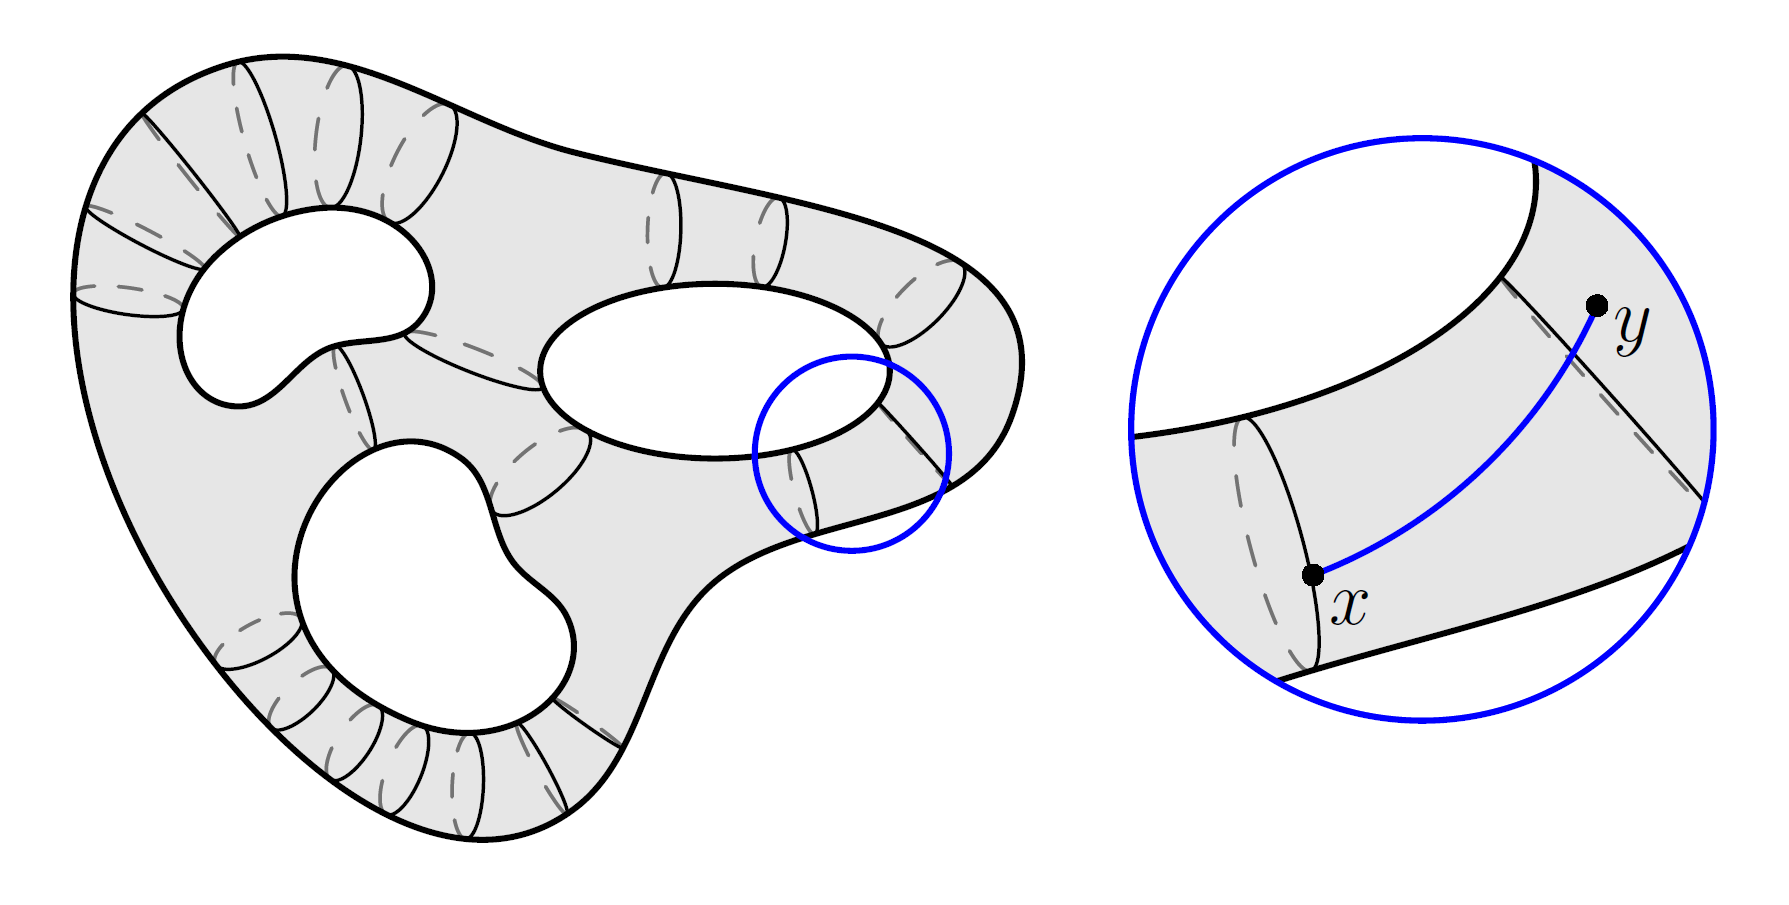
\includegraphics[width = 9.5cm]{16.png}

    \begin{lemma}
        All Riemannian manifolds are locally uniquely geodesic.
    \end{lemma}
\end{frame}

\newpage

\section*{Results}

\begin{frame}{Summary of results}
\footnotesize
\begin{itemize}
    \item \textbf{Internal theory:} Finite nature of convexity, technical statements, hyperplane properties, TPUL and its connection to hyperplanes.

    \item \textbf{Inducing structures:} Freedom of order convexities, Linear and 1-affine space properties, \(n\)-affinity, sufficient conditions for join-commutativity and freedom, attributes of UGS.
    
    \item \textbf{Induced structures:} Polytope interior, convex topology, Riemannian convexity.
\end{itemize}
\end{frame}

\section*{The end}

\begin{frame}
    \centering

    \vspace{12mm}

    {\LARGE Thank you for your attention!}
\end{frame}

\end{document}
